\documentclass[a4paper]{article}
\usepackage[utf8]{inputenc}
\usepackage[left=2cm, right=2cm, top=2cm, bottom=3cm]{geometry}
\usepackage{hyperref}
\usepackage[parfill]{parskip}
\usepackage{tikz}
\usepackage{multicol}
\usepackage{draftwatermark}
\usetikzlibrary{positioning}
\usetikzlibrary{arrows.meta}

\SetWatermarkScale{5}

\newcommand{\todo}[1]{\textsf{TODO: #1}}

\title{License on Blockchain \\[5mm] \large Transferring and Managing Software Licenses on the Ethereum Blockchain\footnote{This white paper acts as documentation for version 1 of the smart contracts deployed on the Ethereum blockchain}}
\author{Alexander Hoppen, Peter Hoppen}
\date{\today, Version 1}

\begin{document}

\maketitle

\bibliographystyle{abbrvdin}

\begin{abstract}
  We present a framework that allows software licenses to be represented on the Ethereum blockchain in a standardised form based on smart contracts, allowing the licenses to be traded without the need of an intermediary while complying with the European laws for trade with used software. A customised wallet has been developed that allows an easy management of the software licenses owned in this framework. Based on the groundwork of this framework, we present new extensions that among others allow a software installation to be activated while guaranteeing that no other installation is used with the same license and not requiring a centralised server maintained by the software manufacturer.
\end{abstract}

\section{Overview}

The trade of used software is currently associated with a considerable organisational overhead. Because of their non-physical nature\footnote{Software licenses are often just represented by a license key. The right to use a software may even just be founded in the software manufacturer's bill.}, it is easy to still use a license even after selling it on. To prevent this issue and allow a trustworthy trade of used software, the following needs to be made sure every time the license is traded:
\begin{enumerate}
  \item The previous owner shall not use the license anymore after the trade has been completed.
  \item The previous owner must not have sold the license to a different person or organisation.
  \item The traded license is genuine and has been issued by the software manufacturer or a certified third party.
  \item The new owner needs to be able to testify that his purchased license is valid by tracing his used license to its original issuing.
\end{enumerate}

Currently, all these checks are performed by \emph{used software traders} that are familiar with the kind of software they are trading so that they can verify the validity of the traded licenses. As part of the process, they will require the seller to sign that he will not be using the software anymore. Furthermore, they keep a record of all completed transfers so that they can trace any license traded by them back to its original issuing, should its genuineness be doubted. 

The above points 1, 2, and 4 are problems that similarly apply to cryptocurrencies like Bitcoin and Ethereum and have been solved for these. In particular, 1 and 2 correspond to the problem of \emph{double spending} where the same coin shall not be able to be spent twice and 4 corresponds to the existence of a \emph{digital ledger} that records the entire transaction history.

In this paper we will introduce an approach that allows software licenses to be represented on the \emph{Ethereum blockchain} and which will thus inherit the advances that have been made in the development of this platform. The key problems that will need to be solved are:
\begin{itemize}
  \item To represent the licenses on the Blockchain in such a way that requirements 1, 2, and 4 are satisfied.
  \item To verify that all licenses represented on the Blockchain are backed by a validly purchased license that is accepted by the software manufacturer (requirement 3).
\end{itemize}

The framework presented in the following shall be called \emph{License on Blockchain (LOB)}.

We will give an overview of the license's representation on the blockchain in section \ref{ch:licenseRepresentationOverview} and describe how the validity of licenses is made sure in section \ref{ch:licenseValidityOverview}. Section \ref{ch:extensionsOverview} will briefly describe new patterns that can be implemented based on top of LOB.

In the following sections we will dive into the smart contract architecture in more detail (section \ref{ch:smartContractArchitecture}) and take a closer look at the license certificate that gives credibility to the LOB licenses (section \ref{ch:licenseCertificate}). Section \ref{ch:wallet} will briefly describe the LOB wallet that runs in a normal internet browser and allows an easy interaction with licenses managed using LOB. In sections \ref{ch:issuingSoftwareLicenses} and \ref{ch:validatingOwnership} we will describe the procedures that need to be performed to issue licenses using LOB and verify their validity. Section \ref{ch:extensions} will touch on new use cases that are enabled by LOB. In the appendix we will finally give a detailed specification of the API of the smart contracts used by LOB.





\subsection{Representation of LOB licenses on Ethereum}
\label{ch:licenseRepresentationOverview}

In order to describe how licenses are managed using LOB, a few terms need to be clarified.

Each separately tradable software \emph{license} on LOB is created as part of an \emph{issuance} by an \emph{issuer} through a smart contract called the \emph{license contract}. An issuance is a single batch of software licenses of the same type (e.g. Microsoft Office Professional 2013) consisting of a fixed number of licenses that can be traded separately. The license contract is a smart contract on the Ethereum blockchain, owned by a single issuer, and manages the different issuances created through it, keeps track of the ownership of single licenses and stores the issuer's identity and liability (see section \ref{ch:licenseValidityOverview} for more information on the last point).

To issue new licenses under a license contract the issuer calls the corresponding function on the license contract\footnote{Invocations of this method by anyone else will be rejected} and passes it a human-readable description and an internal code for the license type, the number of separately tradable licenses that are part of the issuance\footnote{A value of 1 is passed if the licenses can only be traded as a batch}, and the Ethereum address that shall initially own the issued licenses.\footnote{Additional arguments are passed to proof the issuance's validity. These will be described in section \ref{ch:licenseValidityOverview}.}

The issuance is now uniquely identified on the blockchain by an \emph{issuance ID}, consisting of \emph{the license contract's} address and a running \emph{issuance number} of the issuance within the license contract. All separately tradable licenses are assigned to the initial owner's address.

From now on the licenses can be traded without the need for any intermediary. The owner of any license can invoke functions to transfer them to any other Ethereum address which can then pass them on if needed. The license contract is programmed in a way that makes double spending inherently impossible.

To make sure that the license contract behaves correctly and has not been tampered with, an LOB \emph{root contract} creates all license contracts from source code that is hardcoded within it and has been sanctioned by the LOB mother organisation. The creation of a new license contract can be requested by anyone and the root contract will always fulfil the request.

Figure \ref{fig:smartContractHierarchy} gives an overview of the different hierarchy levels in the LOB architecture.

\begin{figure}
  \centering
  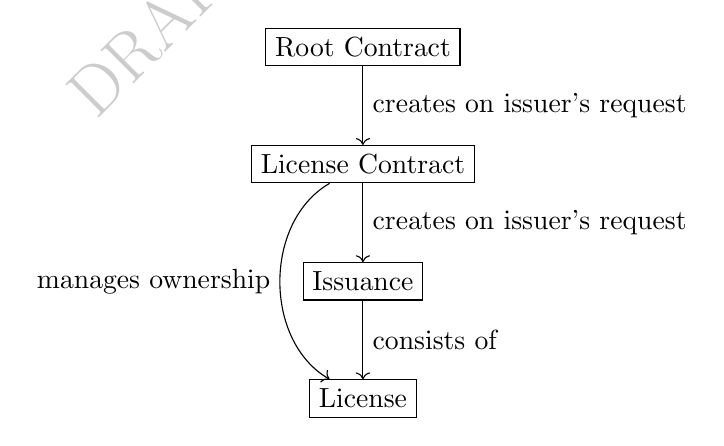
\begin{tikzpicture}
    \node[draw] (rootContract) {Root Contract};
    \node[draw, below=of rootContract] (licenseContract) {License Contract};
    \node[draw, below=of licenseContract] (issuance) {Issuance};
    \node[draw, below=of issuance] (license) {License};
    
    \draw[->] (rootContract) -- node[right] {creates on issuer's request} (licenseContract);
    \draw[->] (licenseContract) -- node[right] {creates on issuer's request} (issuance);
    \draw[->] (issuance) -- node[right] {consists of} (license);
    \draw[->] (licenseContract) edge[bend right=60] node[left] {manages ownership} (license);
  \end{tikzpicture}
  \caption{Hierarchy of components in LOB architecture}
  \label{fig:smartContractHierarchy}
\end{figure}


Section \ref{ch:smartContractArchitecture} will describe the smart contract architecture in more detail and section \ref{ch:wallet} will give an overview of wallet software that has been built to interact with these smart contracts and manage the ownership of licenses using a graphical user interface.





\subsection{Guaranteeing the validity of LOB licenses}
\label{ch:licenseValidityOverview}

In order to give credibility to the issuances managed using LOB, the issuer needs to vouch that the licenses he issues are either backed by genuine \emph{hardcopy licenses}\footnote{Licenses not managed using LOB yet, e.g. a license ownership certificate} or that the issuing is performed by the software manufacturer as an initial sale. 

To do so, the anonymity of the issuer needs to be removed so that he can be made liable should he issue faked licenses. Personal identification on the internet (e.g. for websites using HTTPS or emails via S/MIME) is commonly performed using SSL certificates that are signed by certificate authorities which certify that the owner of an SSL certificate corresponds to the name mentioned in the certificate.
We leverage this existing infrastructure by requiring that the issuer signs his license contract before using it. Should the signature be invalid or the SSL certificate not be trusted, then the license contract and all its issuances are invalid.

In particular, the issuer will sign a \emph{certificate text} stating that he will only use the license contract to issue licenses whose validity he has confirmed by an audit, that he will vouch for the correctness of his confirmation up to a given liability and that he will keep all documents of the confirmation for a given safekeeping period.

Additionally, for every issuance, the issuer needs to specify at which date he performed the audit that confirmed the license's validity and may optionally provide an audit remark describing which steps he took to verify the validity.

Section \ref{ch:licenseCertificate} will describe the contents of the license certificate as well as the other validity features in more detail.





\subsection{Extensions made possible by LOB}
\label{ch:extensionsOverview}

Building on top of the newly created infrastructure, new avenues can be taken. Towards the end of this paper, we will describe a method in which the LOB license is transferred into a \emph{software installation} itself. The basic idea is that every installation of the software will generate an Ethereum address and will only function as long as a valid LOB license is associated with this address. Thus, to activate the software, one needs to transfer the license to that address, reclaiming the license deactivates the installation. Obviously, each license can only be associated with one address. Hence it is impossible to activate multiple installations using the same license or to sell a license while still using it.

Section \ref{ch:extensions} will describe some extensions in some detail.



\section{Smart contract Architecture}
\label{ch:smartContractArchitecture}

In essence, the LOB infrastructure consists of two smart contracts: 
\begin{itemize}
  \item Each \emph{license contract} belongs to a single issuer and manages the ownership of all licenses issued through it. It is the central component to trade licenses.
  \item The \emph{root contract}'s responsibility is to create license contracts on demand and make sure all license contracts share the same implementation and enforce the same legal framework.
\end{itemize}

Both contracts will be described below. For a documentation of the contract's API we refer to the appendix.





\subsection{License contract}
The license contract is the key component which manages the licenses issued by one issuer, their ownership, and gives credibility to these issuances. 

Section \ref{ch:licenseContractCredibility} will describe how a license contract is created and set up so that licenses issued through it can be trusted. Section \ref{ch:licenseContractIssuing} will then go into detail on which steps need to be taken to issue new licenses and in section \ref{ch:licenseContractTransfer} it will be discussed how these licenses can be traded. 





\subsubsection{Credibility of issuances}
\label{ch:licenseContractCredibility}

Before any licenses can be issued or traded, the license contract needs to be created and it needs to be made sure that all issuances under this license contract are performed according to the same rules. This is implemented as a two-step process.

At first, the issuer requests the creation of a new license contract from the root contract, passing it the following parameters:

\begin{itemize}
  \item \textbf{Issuer name}: A human-readable name of the issuer (personal or company name and contact information)
  \item \textbf{Liability}: A free text describing the liability with which the issuer vouches for the validity of the licenses he issues
  \item \textbf{Safekeeping period}: The period of time for which the issuer will keep the documents he used to verify the license's validity safe
  \item \textbf{SSL certificate}: An SSL certificate created for the issuer and signed by a trusted certificate authority
\end{itemize}

Before the newly created license contract can be used to issue licenses, the issuer needs to authenticate himself against the license contract as the owner of the SSL certificate he passed previously and sign a set of rules that makes the trade of LOB licenses compatible with the European laws for the trade of used software.

To do this, the issuer will use the private key of his SSL certificate to sign the \emph{license certificate} that is discussed in detail in section \ref{ch:licenseCertificate}. In summary, it contains the rules mentioned earlier as well as the address of the newly created license contract. The latter is needed to prevent replay attacks where an attacker may reuse the signature of a valid license contract to create a faked copy. It also explains why the creation of the license contract is performed as a two-step process.

Figure \ref{fig:licenseContractCreation} gives a schematic overview of the steps taken to create a new license contract.

\begin{figure}
  \centering
  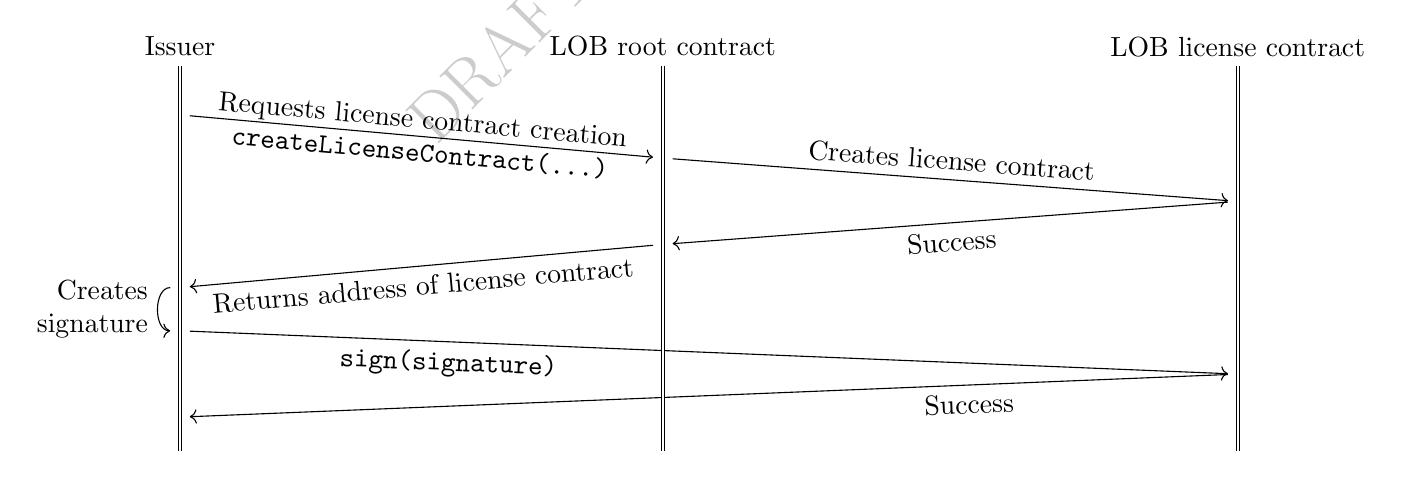
\begin{tikzpicture}[node distance=3mm]
    \node (issuer) {Issuer};
    \node[right=4cm of issuer] (root) {LOB root contract};
    \node[right=4cm of root] (token) {LOB license contract};
    
    \node[below=5mm of issuer] (issuer1) {};
    \node[below=5mm of root] (root1) {};
    \node[below=5mm of token] (token1) {};
    
    \node[below=of issuer1] (issuer2) {};
    \node[below=of root1] (root2) {};
    \node[below=of token1] (token2) {};
    
    \node[below=of issuer2] (issuer3) {};
    \node[below=of root2] (root3) {};
    \node[below=of token2] (token3) {};
    
    \node[below=of issuer3] (issuer4) {};
    \node[below=of root3] (root4) {};
    \node[below=of token3] (token4) {};
    
    \node[below=of issuer4] (issuer5) {};
    \node[below=of root4] (root5) {};
    \node[below=of token4] (token5) {};
    
    \node[below=of issuer5] (issuer6) {};
    \node[below=of root5] (root6) {};
    \node[below=of token5] (token6) {};
    
    \node[below=of issuer6] (issuer7) {};
    \node[below=of root6] (root7) {};
    \node[below=of token6] (token7) {};
    
    \node[below=of issuer7] (issuer8) {};
    \node[below=of root7] (root8) {};
    \node[below=of token7] (token8) {};
    
    \node[below=of issuer8] (issuer9) {};
    \node[below=of root8] (root9) {};
    \node[below=of token8] (token9) {};
    
    \draw[draw, ->] (issuer1) -- node[align=center, sloped] {Requests license contract creation \\ \texttt{createLicenseContract(…)}} (root2);
    \draw[draw, ->] (root2) -- node[above, align=center, sloped] {Creates license contract} (token3);
    \draw[draw, ->] (token3) -- node[below, align=center, sloped] {Success} (root4);
    \draw[draw, ->] (root4) -- node[below, align=center, sloped] {Returns address of license contract} (issuer5);
    \draw[draw, ->] (issuer5) edge[bend right=90] node[left, align=right] {Creates \\ signature} (issuer6);
    \draw[draw, ->] (issuer6) -- node[below, align=center, sloped, pos=0.25] {\texttt{sign(signature)}} (token7);
    \draw[draw, ->] (token7) -- node[below, align=center, sloped, pos=0.25] {Success} (issuer8);
                    
    \draw[double] (issuer) -- (issuer9);
    \draw[double] (root) -- (root9);
    \draw[double] (token) -- (token9);
  \end{tikzpicture}
  \caption{Schematic representation of license contract creation}
  \label{fig:licenseContractCreation}
\end{figure}





\subsubsection{License Issuing}
\label{ch:licenseContractIssuing}

After the license contract has been successfully set up, the issuer may issue licenses through it. Here, two fundamentally different scenarios need to be considered:
\begin{itemize}
  \item The license is issued as part of the original purchase
  \item The license is issued \emph{retroactively} to manage an existing hardcopy license using LOB
\end{itemize}

In the latter case, the issuer will verify that the licensee currently owns the hardcopy license that was previously issued by the software manufacturer. The result of such an audit may be important for any future purchaser to judge the license's validity. Hence the issuer can add a free text \textbf{audit remark} and the \textbf{audit date} at which the audit was performed to any issuance along with the following information:

\begin{itemize}
  \item \textbf{Description}: A human-readable description of the type of license being issued
  \item \textbf{Code}: An unambiguous code for the license type (may be the software manufacturer's name together with the products stock keeping unit (SKU) or another standardised naming scheme)
  \item \textbf{Address of initial owner}: The Ethereum address that initially owns all issued licenses
  \item \textbf{Batch size}: The number of separately tradable licenses issued in this issuance\footnote{A value of 1 is passed if the licenses can only be traded as a batch}
\end{itemize}

When the above data is submitted to the smart contract, the new issuance gets assigned an \emph{issuance number} that is unique within its license contract and can be used to refer to it. The \emph{issuance ID} of an issuance is the address of its licenses contract combined with its issuance number.

In case of a legal dispute it may be necessary for an issuance to be revoked (e.g. because the licensee deliberately deceived the issuer by faking the original license and giving wrong statements). In this case, the license's issuer may revoke the issuance by invoking the corresponding function on the license contract. Any reimbursements associated with this action would need to be decided by a court.

In order to fund future developments of LOB and its maintenance, a small \emph{issuance fee} will be required to be paid towards the LOB mother organisation every time licenses are issued. This fee is set to a default value when the license contract is created but may be adjusted by the LOB mother organisation for each license contract. These fees are collected on the license contract and can only be withdrawn from the LOB mother organisation through the root contract. LOB will not require any fees to be paid for license transfers.

Should the issuer of a license contract suspect that somebody has gained access to the private key of his Ethereum account or wish to deactivate the license contract for whichever reason, he can \emph{disable} it. This will permanently disallow any further license issuings or revokes. 





\subsubsection{License Transfer}
\label{ch:licenseContractTransfer}

After licenses have been issued, they can be traded freely without the need for any intermediary. In particular, this means that the issuer plays no role in any future transfers and licenses may still be traded if the issuer decides to not issue any more LOB licenses.

All balances are kept on a per issuance basis. This means that for each issuance consisting of $n$ individually tradable licenses, it is kept track how these licenses are distributed to different Ethereum addresses. In particular, it means that an address may own licenses of the same type (e.g. Microsoft Office 2016 Standard) that are managed under different issuance IDs. Even if these share the same license code, they are managed separately by LOB since the audits resulting in the issuance of these licenses may have been different and the licenses may thus be revoked independently of each other.

Figure \ref{fig:balanceTally} shows the balance tally for three issuances on the same license contract. Issuances 0 and 2 represent the same type of software but the balances are kept separately.

\begin{figure}
  \begin{multicols}{3}
    \centering
    Issuance Number: 0 \\
    \textbf{Microsoft Office 2016 Standard} \\[3mm]
    
    \begin{tabular}{l|l}
      Address & Balance \\
      \hline
      \texttt{0x34bB4…} & 50 \\
      \texttt{0x79446…} & 25
    \end{tabular}
    
    \columnbreak
    
    Issuance Number: 1 \\
    \textbf{Microsoft Windows 8.1 Enterprise} \\[3mm]
    \begin{tabular}{l|l}
      Address & Balance \\
      \hline
      \texttt{0x79446…} & 100 \\
      \texttt{0xa3500…} & 25 \\
      \texttt{0x94687…} & 75 \\
    \end{tabular}
    
    Issuance Number: 2 \\
    \textbf{Microsoft Office 2016 Standard} \\[3mm]
    \begin{tabular}{l|l}
      Address & Balance \\
      \hline
      \texttt{0x34bB4…} & 15 \\
      \texttt{0x95e24…} & 85
    \end{tabular}
  \end{multicols}
  \caption{Balance tally of a license contract}
  \label{fig:balanceTally}
\end{figure}

In order to transfer a license, the current owner needs to specify the issuance number of the issuance out of which he wants to transfer a license as well as the recipient address and the number of licenses he wants to transfer. Should the amount exceed his balance, the transaction will fail. After successful execution of the transfer transaction, the balance tally for this issuance will be adjusted to credit the transferred licenses to the recipient and deduct them from the sender's balance.

Should any license owner wish to no longer manage the licenses using LOB (e.g. to go back to hardcopy trading for whichever reason), he needs to destroy his LOB license. This is done by transferring the license to the special address \texttt{0x0}.

In addition to the normal transfer, LOB supports an action that allows the current owner to transfer licenses to another address but retain the right to reclaim it at any moment, taking them from the other address's balance without requiring its approval. If address $x$ performs a \emph{temporary transfer} of $n$ licenses to address $y$, we say that $y$ has a \emph{temporary balance} of $n$ and only \emph{temporarily owns} these licenses. Temporarily owned licenses cannot be transferred on.

Licenses who are not temporarily owned form the \emph{proper balance}. The total \emph{balance} of an address is the sum of the temporary balance and the proper balance. If address $x$ can reclaim $n$ licenses from different addresses, we say that $x$ has a \emph{reclaimable balance} of $n$.\footnote{Note that the reclaimable balance does not contribute to the total balance since these licenses are not currently associated to the address.}

The main use case for this kind of transfer is to allow individual installations to be \emph{activated} using LOB licenses. In a nutshell, the installation will generate an Ethereum address and only function if this address has a non-zero balance of the right license type. To activate the installation, a license can be temporarily transferred to this address to activate the installation and if the installation shall be deactivated, the license can be reclaimed. Section \ref{ch:installationActivation} describes the procedure in more detail.





\subsubsection{Balance lookup}
\label{ch:licenseContractBalanceLookup}

Given an Ethereum address, it needs to be easily possible to check which licenses are owned by that address. In the most basic case, if the address and an issuance ID is known, the balance and temporary balance of that address can be queried from the license contract. Additionally, the license contract keeps track of all license transfers through events\footnote{Also known as logs} from which the entire transfer history of a given issuance can be reconstructed. Figure \ref{fig:transferHistory} shows the transfer history of a given issuance as a graph.

\begin{figure}
  \centering
  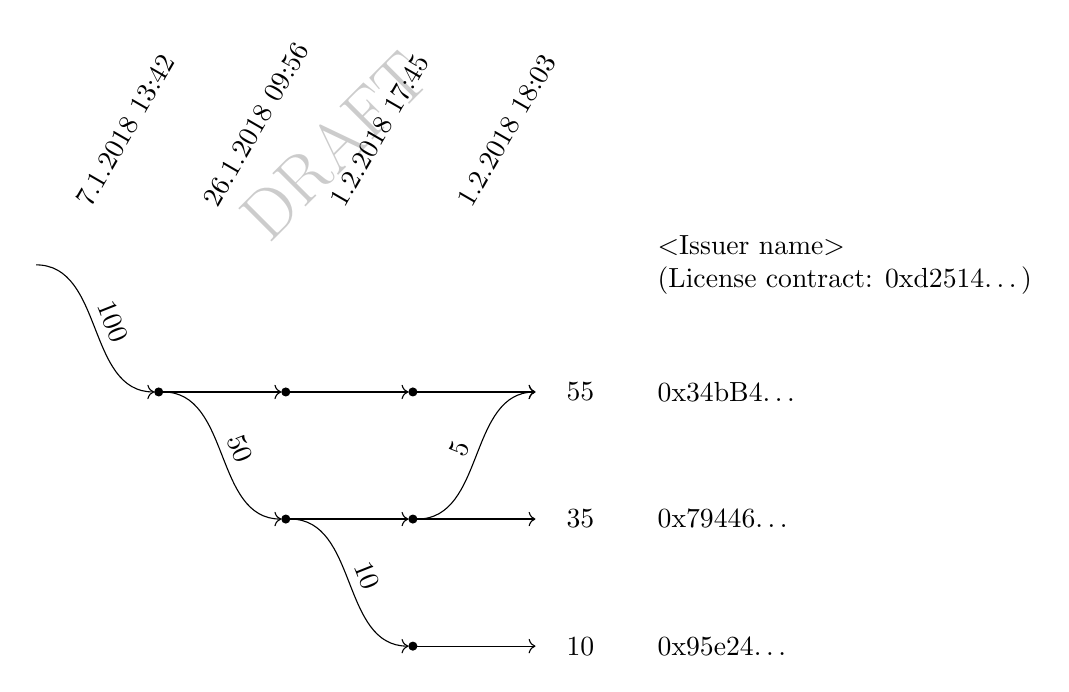
\begin{tikzpicture}[node distance=1.5cm,
    coordinate/.style={draw, shape=circle, inner sep=0mm, minimum size=1mm, fill=black},
    unusedCoordinate/.style={shape=circle, inner sep=0mm, minimum size=1mm},
  ]
    \node[unusedCoordinate] (0_0) {};
    \node[unusedCoordinate, below=of 0_0] (0_1) {};
    \node[unusedCoordinate, below=of 0_1] (0_2) {};
    \node[unusedCoordinate, below=of 0_2] (0_3) {};
    
    \node[unusedCoordinate, right=of 0_0] (1_0) {};
    \node[coordinate, right=of 0_1] (1_1) {};
    \node[unusedCoordinate, right=of 0_2] (1_2) {};
    \node[unusedCoordinate, right=of 0_3] (1_3) {};
    
    \node[unusedCoordinate, right=of 1_0] (2_0) {};
    \node[coordinate, right=of 1_1] (2_1) {};
    \node[coordinate, right=of 1_2] (2_2) {};
    \node[unusedCoordinate, right=of 1_3] (2_3) {};
    
    \node[unusedCoordinate, right=of 2_0] (3_0) {};
    \node[coordinate, right=of 2_1] (3_1) {};
    \node[coordinate, right=of 2_2] (3_2) {};
    \node[coordinate, right=of 2_3] (3_3) {};
    
    \node[unusedCoordinate, right=of 3_0] (4_0) {};
    \node[unusedCoordinate, right=of 3_1] (4_1) {};
    \node[unusedCoordinate, right=of 3_2] (4_2) {};
    \node[unusedCoordinate, right=of 3_3] (4_3) {};
    
    \node[right=1mm of 4_0, align=left, minimum width=7mm] (balance_0) {};
    \node[right=1mm of 4_1, minimum width=7mm] (balance_1) {55};
    \node[right=1mm of 4_2, minimum width=7mm] (balance_2) {35};
    \node[right=1mm of 4_3, minimum width=7mm] (balance_3) {10};
    
    \node[right=5mm of balance_0, align=left] (label_0) {\textless Issuer name\textgreater \\ (License contract: 0xd2514…)};
    \node[right=5mm of balance_1] (label_1) {0x34bB4…};
    \node[right=5mm of balance_2] (label_2) {0x79446…};
    \node[right=5mm of balance_3] (label_3) {0x95e24…};
    
    \node[above right=5mm and 7.5mm of 0_0, rotate=60] (time_0) {7.1.2018 13:42};
    \node[above right=5mm and 7.5mm of 1_0, rotate=60] (time_0) {26.1.2018 09:56};
    \node[above right=5mm and 7.5mm of 2_0, rotate=60] (time_0) {1.2.2018 17:45};
    \node[above right=5mm and 7.5mm of 3_0, rotate=60] (time_0) {1.2.2018 18:03};
    
    \path[->] (0_0) edge[out=0, in=180] node[above, sloped] {100} (1_1);
    
    \path[->] (1_1) edge[out=0, in=180] node[above, sloped] {} (2_1);
    \path[->] (1_1) edge[out=0, in=180] node[above, sloped] {50} (2_2);
    
    \path[->] (2_1) edge[out=0, in=180] node[above, sloped] {} (3_1);
    \path[->] (2_2) edge[out=0, in=180] node[above, sloped] {} (3_2);
    \path[->] (2_2) edge[out=0, in=180] node[above, sloped] {10} (3_3);
    
    \path[->] (3_1) edge[out=0, in=180] node[above, sloped] {} (4_1);
    \path[->] (3_2) edge[out=0, in=180] node[above, sloped] {} (4_2);
    \path[->] (3_3) edge[out=0, in=180] node[above, sloped] {} (4_3);
    \path[->] (3_2) edge[out=0, in=180] node[above, sloped] {5} (4_1);
  \end{tikzpicture}
  \caption{Transfer history graph of an issuance}
  \label{fig:transferHistory}
\end{figure}

Since all license contracts are created from a fixed set of known root contracts and the license contract exposes all used issuance numbers, one could theoretically iterate through all issuance IDs and retrieve the address's balance for these.

For most issuances, however, the balance for a given address will be zero. To avoid unnecessary computation, the license contract keeps track for which issuances an address has ever owned licenses. This list of \emph{relevant issuances} will include all issuance numbers of issuances for which an address currently has a non-zero balance or used to have a non-zero balance but has since passed all licenses on. It has proven that this data structure strikes a good balance between ruling out the majority of irrelevant issuances and being cheap\footnote{In terms of computational power} to keep track of.

Similarly, it needs to be possible to determine if a given address can reclaim licenses from other addresses and if so, these addresses need to be determined. Therefore, for each address and issuance number the license contract keeps track of all addresses to which licenses have ever been transferred temporarily. This list is also never cleared and only appended to and thus an over-approximation of the actual set of addresses from which licenses can be reclaimed, but has the same desirable properties that are described above.





\subsection{Root contract}
\label{ch:rootContract}

Since all license contracts are created from a fixed set of known root contracts and the license contract exposes all used issuance numbers, one could theoretically iterate through all issuance IDs and retrieve the address's balance for these.

For most issuances, however, the balance for a given address will be zero. To avoid unnecessary computation, the license contract keeps track for which issuances an address has ever owned licenses. This list of \emph{relevant issuances} will include all issuance numbers of issuances for which an address currently has a non-zero balance or used to have a non-zero balance but has since passed all licenses on. It has proven that this data structure strikes a good balance between ruling out the majority of irrelevant issuances and being cheap\footnote{In terms of computational power} to keep track of.

Similarly, it needs to be possible to determine if a given address can reclaim licenses from other addresses and if so, these addresses need to be determined. Therefore, for each address and issuance number, the license contract keeps track of all addresses to which licenses have ever been transferred temporarily. This list is also never cleared and only appended to and thus an over-approximation of the actual set of addresses from which licenses can be reclaimed, but has the same desirable properties that are described above.





\section{License Certificate}
\label{ch:licenseCertificate}

The license certificate is the key legal building block that guarantees that licenses represented in the LOB framework are either issued during its initial purchase or backed by a genuine hardcopy license that is no longer traded outside the LOB framework.

In essence, the license certificate consists of three key statements which the issuer has to acknowledge by signing the license certificate using his SSL private key before issuing licenses.

\begin{enumerate}
  \item The issuer will only issue licenses for which he has been assured by the license owner in an audit that the hardcopy licenses have been purchased correctly, have not been sold on, and are not managed using LOB or another similar scheme yet. All documents that were inspected during the audit will be kept safe by the issuer for the safekeeping period that was specified during the license contract's creation
  \item The issuer will oblige the recipient of the LOB licenses to only transfer the license using LOB and require the same from everyone he transfers the licenses to. Should the recipient wish to pass the hardcopy license on, he needs to destroy the LOB license first.
  \item If the above requirements have been fulfilled by the license's owner, the issuer will uphold the license certificate for everyone to whom the licenses have been transferred and vouch for the licenses validity up to the liability he has specified during the license contract's creation.
\end{enumerate}



\section{LOB wallet}
\label{ch:wallet}

The interaction with the two smart contracts described so far could be done through standard wallet software that allows generic interactions with smart contracts by invoking the functions described in sections \ref{ch:licenseContractAPI} and \ref{ch:rootContractAPI} directly, but the easiest way to interact with these is the \emph{LOB Wallet}. This wallet will automatically present the user his current balance of licenses in a graphical user interface and allow easy transfers of these licenses while keeping track of the transfer's confirmation status on the Ethereum blockchain. This Dapp\footnote{Distributed application} is implemented as a locally running reactive webpage that interacts with Ethereum using the officially sanctioned open source web3.js framework.

\subsection{Overview}

For issuers, the wallet will guide the user through the process of creating their own license contract, informing them on which information he needs to enter, making sure that the SSL certificate is in the correct format and help them generate the signature to sign the license contract. From there on, the wallet will offer the issuer a set of predefined software types for which licenses can be issued while giving him the option to specify the license type's description and code himself.

For license owners, the wallet will show a list of licenses owned by him, validating that their license contract is sound, allowing him to view all information he might consider to judge the license's trustworthiness (including the issuer's liability and the license's transfer history). From there, he is also able to easily transfer the licenses or reclaim licenses he has previously transferred temporarily.

Upon visiting the website that hosts the LOB wallet\footnote{\url{https://wallet.lob.alexhoppen.de} \todo{Enter real URL}}, the user will be required to enable Web3 functionality for his browser so that the wallet can communicate with the Ethereum blockchain. The easiest and recommended way is to install the MetaMask\footnote{\url{https://metamask.io}} plugin for the user's browser, but using any other Web3-capable browser like Mist\footnote{Mist is the official Dapp browser for Ethereum, \url{https://github.com/ethereum/mist/releases}} is also supported.

After installation of MetaMask, the user will generate an Ethereum address under which he can receive LOB licenses. If he wishes to transfer licenses, he needs to purchase Ether and deposit them on his account so that he can pay the transaction fees towards the miners that are required by the Ethereum network.

\subsection{Technical details}

The LOB Wallet runs entirely in the user's browser and never transfers any data to LOB's servers. All external communication is done transparently through the Ethereum blockchain. Should the user wish, he can download the wallet and run it locally.

The entire communication with the Ethereum blockchain is done through the web3.js\footnote{\url{https://github.com/ethereum/web3.js}} framework which may be injected into common browsers using the MetaMask plugin or is natively provided by the official Ethereum Dapp browser Mist.

Upon launching the LOB Wallet, it scans the Ethereum blockchain for licenses owned by any of the user's addresses as described in section \ref{ch:licenseContractBalanceLookup}, starting the search at a fixed set of hardcoded root contracts.

After the initialisation of the wallet with the current balance, the LOB wallet listens for events which may change the current state and reactively updates its state (by e.g. updating balances on an incoming license transfer). Data that is known not to change (like a license contract's SSL certificate) is persistently stored in the browser so that the information can be retrieved from the local cache the next time the wallet is launched and bandwidth to the Ethereum network is saved.

For each license that is displayed to the user, the wallet automatically verifies the integrity of the license contract's signature and displays the issuer's liability and all SSL certificate details to the user should he further wish to examine the certificate's trustworthiness.





\section{Issuing software licenses}
\label{ch:issuingSoftwareLicenses}

The following shall describe the process of issuing an LOB license in more detail. 

\subsection{Phase 1: Initial license validation}

In a first step, the issuer of the license needs to ensure that the licensee actually owns the software license whose management shall from now on be performed using LOB. For this, multiple scenarios are possible, including the following:
\begin{itemize}
  \item The LOB license is issued upon purchase of the actual license. The seller of the software license knows by definition that the purchaser will own the license on purchase and can simply issue the LOB license instead of a hardcopy license as part of fulfilling the purchase contract.

  \item Used software traders already have well-established procedures to verify that the instance selling used software to them is not using it anymore. When the used software trader resells the software, it can issue an LOB license as if it were a software manufacturer.

  \item Similarly, any trustworthy third party may perform the validations used software traders perform at the moment, but without purchasing the licenses that shall from now on be managed using LOB. Instead, the third party simply issues the LOB license to the current hardcopy license owner. One crucial aspect of validation the issuer has to perform is that it must certify that the license is not managed using LOB (or any similar system) yet, as to prevent the issuing of multiple LOB licenses for the same hardcopy license. Furthermore, the issuer needs to ensure that the licensee does not sell the hardcopy license without invalidating the LOB license first. This is done by including a paragraph in the license contract's certificate (which is signed by the issuer) that obliges every LOB purchaser to not sell the license outside the LOB framework without destroying its LOB counterpart first.
\end{itemize}

\subsection{Phase 2: Blockchain transactions}

After the issuer has verified that he wants to issue an LOB license as described in the previous section, he performs the following steps:

\begin{enumerate}
  \item If the issuer does not have a license contract yet, it generates one.
  \item He determines a unique code for the license type to be managed using LOB. This may be the SKU of the software manufacturer or another standardised naming scheme.
  \item He composes a human-readable description for the license type.
  \item He determines if the licenses can be traded separately or only in bulk. If the licenses can only be traded in bulk the number of separately tradable licenses is 1 and the batch size needs to be noted in the description and code.
  \item If a license audit was conducted in phase 1, the issuer composes a remark describing his actions and result of the audit and notes the date and time at which the audit was performed.
  \item He asks the licensee for his Ethereum address. If the licensee does not have an Ethereum address yet, he can create one by initialising the LOB wallet as described in section \ref{ch:wallet}\footnote{The licensee does not need to deposit Ether on his address to receive the license. Only to trade them Ethers are needed to cover network transaction costs.}.
  \item The issuer invokes \texttt{issueLicense(…)} on his license contract with the parameters he has just determined using the LOB wallet.
  \item After the transaction gets mined, the licensee can verify his license ownership using the LOB wallet.
\end{enumerate}





\section{Validating the ownership of a software license}
\label{ch:validatingOwnership}

Verifying all integrity concerns of token contracts on the blockchain is neither advisable due to the high transaction costs to perform expensive computations, nor is it necessary. Some verification steps don't have a single “right” answer but the licensee needs to judge for himself which requirements apply (such as which certificate authorities to trust or which liability to require). Wallet software has to guide the user through these validation steps and simplify information as much as possible while still allowing the user to view all information.

The following list shall be a guideline on what checks must be performed to verify that someone owns the LOB license he claims to own. All of the following steps can be performed offline and do not require gas for any transaction to be performed on the blockchain.

\begin{itemize}
  \item Verify that the other party owns the private key of the Ethereum address he claims to possess by giving him a message to sign and verify that the signature can be decrypted using the address's public key
  \item Determine the issuance ID (license contract address and issuance number) to which the license in question belongs
  \item Call \texttt{balance(…)} with the issuance number and the licensee's address on the license contract and verify that a number of licenses matches (or exceeds) the claimed amount
  \item Check that the issuance has not been revoked
  \item Check that the license name describes the type of license the licensee claims to own
  \item Check that the data returned by \texttt{issuerSSLCertificate()} is a valid SSL certificate
  \item Verify that the name in the issuer's SSL certificate matches the name returned by \texttt{issuerName()}
  \item Judge whether the certificate authority that issued the certificate is trustworthy and has the required security level
  \item Check if the issuer's SSL certificate has been revoked
  \item Verify that the data returned by \texttt{signature()} is a valid signature of the text returned by \texttt{certificateText()} using the certificate returned by \texttt{issuerSSLCertificate()}
  \item Check that the liability is sufficient
\end{itemize}

The wallet described in section \ref{ch:wallet} guides the user through these verification steps. It automatically verifies the license contract's signature and provides the user with a list of decisions he needs to make for himself. For example, there is no “right” decision for which liability is required for a license issuance and the user needs to judge for himself if what the issuer provided in the free text format satisfies his needs. Furthermore, the SSL certificate may have been issued for the issuer's website and contain the website's URL as its common name. It will thus not match the name returned by \texttt{issuerName()} but the user may still decide to trust the issuance if the domain and issuer name match.



\section{Extensions}
\label{ch:extensions}

In this section we want to highlight three extensions that can be built on top of LOB without requiring any modification to the framework that was proposed so far.

\subsection{Activating and deactiviating installations using LOB licenses}
\label{ch:installationActivation}

Even if licenses are managed using LOB, it does not prevent a license owner from activating multiple installations using the same license or keeping an existing installation activated while passing the license that was used to activate said installation, on, even though it is not allowed by license terms. In this section we will describe a method that allows installations to be activated directly using license's representation in LOB and disallowing any other uses of this license while upholding an installation's activation.

For this, the software installation will generate an Ethereum address when it is being installed and periodically poll that address's balance. The installation will consider itself activated if an appropriate license\footnote{Licenses which contain a fixed SKU as the license's code and are issued through license contract's owned by the software manufacturer himself or some trusted third party} is owned by its address. Since the license can only be owned by a single address, the same license cannot activate another installation (which would require it to be also owned by the other installation's address, which is different) or passed on to a new owner (since this owner would need to own the license under his address).

In practice, after being installed, the software will ask the user to \emph{temporarily transfer} an appropriate license to the Ethereum address it has just generated. Once the user has submitted this transfer and the transaction is mined, the installation will pick up its non-zero license balance and be activated. Until such time, it may operate in a trial mode or give the user a grace period of several days to submit the transaction. Should the user wish to use the license in another way (e.g. to activate a different installation or sell it on), he can \emph{reclaim} the license from the installation's address. The installation will notice the non-zero balance next time it checks\footnote{e.g. on the next launch} and deactivate itself.

Notice that in the entire scheme the installation's address never submits any transactions and is thus neither required to own any Ether nor is its private key ever needed.\footnote{We still recommend the software to keep track of the private key so that in case the user transferred a license to the address non-temporarily, the installation can show the private key to the user who can then deposit Ether on it and submit a transaction that passes the license back to his original address.}

We would also like to highlight that a software manufacturer does not need to operate any servers to adopt the above method since all management is done on the Ethereum blockchain. It will even continue to work, should the manufacturer go out of business or decide to no longer support a software product.





\subsection{Certification of license issuers}
\label{ch:licenseIssuerValidation}

To simplify the judgement of whether or not an issuer is trustworthy (checking its liability, SSL certificate, internal standards), an independent institution can verify license issuers, giving them some status of trustworthiness. This list could be managed on a central address on the Ethereum blockchain but is other than by wallet integration not affiliated with LOB.





\subsection{Purchase contract}
\label{ch:purchaseContract}

To avoid the issue where one party transfers the LOB license to be traded but the other does not pay the agreed amount (or vice versa), the trading parties may agree to set up a smart contract that takes the role of an escrow: Only after the seller of the license has transferred the license to this smart contract and the purchaser has transferred the agreed price (in Ether) to the smart contract can the purchaser retrieve the licenses from the escrow and the seller take the deposited money. No adjustment of LOB's smart contracts is necessary for this.





\clearpage

\section{Appendix}

\subsection{License contract API}
\label{ch:licenseContractAPI}

\subsubsection{Liability and issuer identification}

\begin{itemize}
  \item \texttt{function issuerName() constant returns (string)}
  \begin{itemize}
    \item Returns a human-readable name that unambiguously describes the person or organisation issuing licenses via this contract.
    \item This should to the most possible extent match the name in the \texttt{issuerSSLCertificate}. Ideally, \texttt{issuerSSLCertificate} is a Class 3 EV certificate and issued to exactly this name. Should \texttt{issuerSSLCertificate} reference a URL, this URL should obviously refer to the website of this person or organisation.
    \item It is not validated on the blockchain if this invariant holds because the computational cost would be too high. The LOB Wallet performs these validations.
  \end{itemize}
  
  \item \texttt{function liability() constant returns (string)}
  \begin{itemize}
    \item Returns he liability the issuer guarantees for each issuance.
  \end{itemize}
  
  \item \texttt{function safekeepingPeriod() constant returns (uint8)}
  \begin{itemize}
    \item Returns the number of years all documents related to the audit will be kept safe by the issuer.
  \end{itemize}
  
  \item \texttt{function issuerSSLCertificate() constant returns (bytes)}
  \begin{itemize}
    \item Returns the SSL certificate that identifies the owner of this license contract. The private key of this certificate is used to generate the signature for this license contract. See the documentation of \texttt{issuerName} for the  constraints on how the name in this certificate should match the name  stored in \texttt{issuerName}.
    \item The certificate needs to be PKCS\#12 encoded and encrypted with an empty password.
    \item It is not verified on the blockchain if this certificate is in the correct format because the computational cost would be too high. The LOB Wallet performs this validation.
  \end{itemize}
  
  \item \texttt{function issuer() constant returns (address)}
  \begin{itemize}
    \item Returns the address that is allowed to issue and revoke issuances and disable the license contract.
  \end{itemize}
  
  \item \texttt{function signature() constant returns (bytes)}
  \begin{itemize}
    \item Returns the signature generated by signing the certificate text of this license contract using the private key of \texttt{issuerSSLCertificate}.
    \item This is a SHA-256 digest of the certificate text signed using the private key of the SSL certificate. It can be generated using OpenSSL with the following command: \\\texttt{openssl dgst -sha256 -sign privateKey.key -hex CertificateText.txt}.
  \end{itemize}
\end{itemize}

\subsubsection{License contract creation}

\begin{itemize}
  \item \texttt{function LicenseContract(address \_issuer, string \_issuerName, string \_liability, \\uint8 \_safekeepingPeriod, bytes \_issuerSSLCertificate, uint128 \_fee)}
  \begin{itemize}
    \item Creates a new license contract.
    \item The sender of this message becomes the LOB root.
    \item New license contracts should only be created via an LOB root contract and this method should thus never be called directly.
    \item \texttt{\_issuer}: The address that will be allowed to issue licenses via this contract
    \item \texttt{\_issuerName}: The name of the person or organisation that will issue licenses via this contract. See documentation of \texttt{issuerName()} for more information.
    \item \texttt{\_liability}:  The liability the issuer guarantees for each issuance
    \item \texttt{\_safekeepingPeriod}: The number of years all documents related to the audit will be kept by the issuer
    \item \texttt{\_issuerSSLCertificate}: An SSL certificate created for the person or organisation that will issue licenses via this contract. See documentation of \texttt{issuerSSLCertificate()} for more information.
    \item \texttt{\_issuanceFee}: The fee that is required to be paid for each license issuance in Wei. May be changed later.

  \end{itemize}
  
  \item \texttt{function certificateText() constant returns (string)}
  \begin{itemize}
    \item Builds the certificate text by filling custom placeholders into a template certificate text.
    \item This is the text that needs to be signed to generate the signature for the \texttt{sign} method.
    \item Returns the certificate text template with placeholders instantiated by the given parameters
  \end{itemize}
  
  \item \texttt{function sign(bytes \_signature)}
  \begin{itemize}
    \item Signs the license contract, verifying that the private key of this contract's issuer's address is owned by the owner of the private key for \texttt{issuerSSLCertificate} and that the issuer will comply with the LOB rules.
    \item The signature shall sign the text returned by \texttt{certificateText()} using the private key belonging to \texttt{issuerSSLCertificate}. It must be a SHA-256 digest of the certificate text signed using the private key of the SSL certificate and can be generated using OpenSSL with the following command: \\\texttt{openssl dgst -sha256 -sign privateKey.key -hex CertificateText.txt}
    \item Prior to signing the license contract, licenses cannot be issued.
    \item It is not verified on the blockchain if the signature is valid or well-formed due to the high computational cost. The LOB Wallet performs this validation.
    \item The signature cannot be overwritten once it is set.
    \item \texttt{\_signature}: The signature with which to sign the license contract
  \end{itemize}
  
  \item \texttt{event Signing()}
  \begin{itemize}
    \item Fired when the smart contract gets signed.
  \end{itemize}
\end{itemize}

\subsubsection{License issuing}

\begin{itemize}
  \item \texttt{function issueLicense(string licenseDescription, string licenseCode, address \\ initialOwnerAddress, uint64 numLicenses, string auditRemark, uint32 auditTime) payable}
  \begin{itemize}
    \item Issues new LOB licenses. The following conditions must be satisfied for this function to succeed:
    \begin{itemize}
      \item The function must be called by the issuer
      \item The license contract needs to be signed
      \item The license contract must not be disabled
      \item The issuance fee must be transmitted together with this message
      \item LOB must not have taken over control of the license contract
    \end{itemize}
    \item It will create a new issuance. The event \texttt{Issuing} is fired with the issuance number of the newly created issuance.
    \item \texttt{licenseDescription}: A human-readable description of the license type
    \item \texttt{licenseCode}: An unambiguous code for the license type
    \begin{itemize}
      \item This could be the SKU of the product used by the software manufacturer together with the manufacturer's name or a free text description
    \end{itemize}
    \item \texttt{initialOwnerAddress}: The address that shall initially own all the licenses
    \item \texttt{numLicenses}: The number of separately tradable licenses to be issued
    \item \texttt{auditRemark}: A free text field containing the result of the license audit
    \item \texttt{auditTime}: The time at which the audit was performed
    \begin{itemize}
      \item Unix timestamp (seconds since 1970-01-01 00:00:00 +0000)
    \end{itemize}
  \end{itemize}
  
  \item \texttt{event Issuing(uint256 issuanceNumber)}
  \begin{itemize}
    \item Fired when a new issuance is created.
    \item \texttt{issuanceNumber}: The issuance number of the newly created issuance
  \end{itemize}
  
  \item \texttt{function issuanceFee() constant returns (uint128)}
  \begin{itemize}
    \item Returns the fee in Wei that is required to be paid for every license issuance.
    \item The fees are collected in the license contract and may be withdrawn by the LOB root.
  \end{itemize}
  
  \item \texttt{function revoke(uint256 issuanceNumber, string revocationReason)}
  \begin{itemize}
    \item Revokes the given issuance, disallowing any further license transfers (including temporary transfers) or reclaims. 
    \item This action cannot be undone.
    \item This can be performed by the issuer if control has not been taken over for this license contract and the license contract has not been disabled. If control has been taken over, the manager may revoke licenses even if the license contract has been disabled.
    \item \texttt{issuanceNumber}: The issuance that shall be revoked
    \item \texttt{revocationReason}: A free text explaining why the issuance is revoked
  \end{itemize}
  
  \item \texttt{event Revoke(uint256 issuanceNumber)}
  \begin{itemize}
    \item Fired when an issuance gets revoked.
    \item \texttt{issuanceNumber}: The issuance that gets revoked
  \end{itemize}
\end{itemize}

\subsubsection{Balance retrieval}

\begin{itemize}
  \item \texttt{function issuances(uint256 issuanceNumber) constant returns (Issuance)}
  \begin{itemize}
    \item Returns an \texttt{Issuance} struct for the issuance with the given issuance number
    \item The struct consists of the following fields:
    \begin{itemize}
      \item \texttt{description} (string): A human-readable description of the type of license managed by this issuance
      \item \texttt{code} (string): An unambiguous code for the type of license this issuance manages
      \item \texttt{originalSupply} (uint64): The number of licenses originally issued in this issuance
      \item \texttt{auditTime} (uint32): The date at which the audit was performed
      \item \texttt{auditRemark} (string): A free text field containing the result of the license audit
      \item \texttt{revoked} (bool): Whether or not this issuance has been revoked, thus not allowing any more license transfers or reclaims
      \item \texttt{revocationReason} (string): If the license has been revoked, a free text filled by the issuer explaining why he as revoked the issuance
    \end{itemize}
  \end{itemize}
  
  \item \texttt{function issuancesCount() constant returns (uint256)}
  \begin{itemize}
    \item Returns the number of issuances created using this license contract
    \item This is an upper bound (exclusively) on the issuance number for \texttt{issuances(issuanceNumber)}
  \end{itemize}
  
  \item \texttt{function relevantIssuances(address owner, uint256 index) returns (uint256)}
  \begin{itemize}
    \item Returns the \texttt{index}th relevant address for which \texttt{owner} may own licenses
    \item The purpose of this cache is to find an over-approximation of the license numbers for which a given address currently owns licenses. To keep computational cost low, this list is never cleared. Hence, the existence of an issuance number in it does not guarantee that the address currently owns licenses of this type. Since it is only appended to, issuance numbers may occur multiple times.
    \item \texttt{owner}: The owner for which relevant issuances shall be determined
    \item \texttt{index}: The \texttt{index}th relevant issuance shall be retrieved
    \begin{itemize}
      \item Must be smaller than \texttt{relevantIssuancesCount(owner)}
    \end{itemize}
  \end{itemize}
  
  \item \texttt{function relevantIssuancesCount(address owner) constant returns (uint256)}
  \begin{itemize}
    \item Determines the number of issuances relevant for the given owner that can be retrieved using \\\texttt{relevantIssuances(owner, i)} where \texttt{i < relevantIssuancesCount(owner)}.
    \item Note that because \texttt{relevantIssuances} is an over-approximation, it may contain duplicate and outdated entries. Thus, the number of actually relevant issuances for this owner may be smaller than the number returned by this method.
    \item Returns an upper bound (exclusive) \texttt{i} that can be used when accessing \texttt{relevantIssuances(owner, i)}
    \item \texttt{owner}: The owner for which relevant issuances shall be determined
  \end{itemize}
  
  \item \texttt{function temporaryLicenseHolders(uint256 issuanceNumber, \\address originalOwner, uint256 index) constant returns (address)}
  \begin{itemize}
    \item Retrieves the \texttt{index}th address from which licenses may be reclaimable by \texttt{originalOwner}. The maximum index can be determined using \texttt{temporaryLicenseHoldersCount}.
    \item \texttt{temporaryLicenseHolders} is a list of addresses to which licenses have been transferred temporarily by \texttt{originalOwner}. It is an auxiliary list to quickly determine a superset of the addresses from which licenses may be reclaimed while being computationally cheap to manage.
    \item Whenever \texttt{x} has temporarily transferred a licenses to \texttt{y}, \texttt{y} will be in \texttt{temporaryLicenseHolders[x]}. The list is  never cleared, thus the existence of an address in the list does not guarantee that a reclaim is possible (e.g. if the licenses has already been reclaimed). Addresses may occur multiple times in the list since it is only appended to.
    \item Returns an address from which \texttt{originalOwner} may be able to reclaim licenses of the given issuance number
    \item \texttt{issuanceNumber}: The issuance for which the temporary license holders shall be determined
    \item \texttt{originalOwner}: The address that would like to reclaim licenses
    \item \texttt{index}: The array index that shall be retrieved. Must be smaller than the count returned by \texttt{temporaryLicenseHoldersCount(issuanceNumber, originalOwner)}
  \end{itemize}
  
  \item \texttt{function temporaryLicenseHoldersCount(uint256 issuanceNumber, address originalOwner) \\constant returns (uint256)}
  \begin{itemize}
    \item Determines the number of addresses from which \texttt{originalOwner} may be able to reclaim licenses of issuance \texttt{issuanceNumber}. These addresses can be retrieved using \texttt{temporaryLicenseHolders}.
    \item Note that because \texttt{temporaryLicenseHolders} is an over-approximation, it may contain duplicate entries and is never cleared. Thus, the number of addresses \texttt{originalOwner} is able to reclaim licenses from is likely lower than the count returned by this function.
    \item Returns an upper bound (exclusive) on the index for \texttt{temporaryLicenseHolders}
    \item \texttt{issuanceNumber}: The issuance for which the addresses from which licenses may be reclaimable shall be determined
    \item \texttt{originalOwner}: The address that would like to reclaim licenses
  \end{itemize}
  
  \item \texttt{function balance(uint256 issuanceNumber, address owner) constant returns (uint64)}
  \begin{itemize}
    \item Returns the number of licenses of a given issuance owned by \texttt{owner} including licenses that are only owned temporarily.
    \item \texttt{issuanceNumber}: The issuance for which the number of licenses owned by \texttt{owner} shall be determined
    \item \texttt{owner}: The address for which the balance shall be determined
  \end{itemize}
  
  \item \texttt{function temporaryBalance(uint256 issuanceNumber, address owner) \\constant returns (uint64)}
  \begin{itemize}
    \item Returns the number of licenses of a given issuance temporarily owned by \texttt{owner} and which thus may be reclaimed by a different address (i.e. the number of licenses that are not properly owned by \texttt{owner}).
    \item \texttt{issuanceNumber}: The issuance for which the balance shall be determined
    \item \texttt{owner}: The address for which the balance shall be determined
  \end{itemize}
  
  \item \texttt{function temporaryBalanceReclaimableBy(uint256 issuanceNumber, address owner, \\address reclaimer) constant returns (uint64)}
  \begin{itemize}
    \item Returns the number of licenses of a given issuance owned by \texttt{owner} but which may be reclaimed by \texttt{reclaimer}.
    \item \texttt{issuanceNumber}: The issuance for which the balance shall be determined
    \item \texttt{owner}: The address that temporarily owns the licenses
    \item \texttt{reclaimer}: The address that is allowed to reclaim the licenses from \texttt{owner}
  \end{itemize}
\end{itemize}

\subsubsection{License transfer}

\begin{itemize}
  \item \texttt{function transfer(uint256 issuanceNumber, address to, uint64 amount)}
  \begin{itemize}
    \item Transfers \texttt{amount} licenses of the given issuance from the sender's address to \texttt{to}. \texttt{to} becomes the new proper owner of these licenses.
    \item This requires that:
    \begin{itemize}
      \item The sender properly owns at least \texttt{amount} licenses of the given issuance (transferring temporary balance is not allowed)
      \item The issuance has not been revoked
    \end{itemize}
    \item Upon successful transfer, this fires the \texttt{Transfer} event with \texttt{temporary} set to \texttt{false}.
    \item \texttt{issuanceNumber}: The issuance to which the licenses to be transferred belong
    \item \texttt{to}: The address the licenses shall be transferred to
    \item \texttt{amount}: The number of licenses that shall be transferred
  \end{itemize}
  
  \item \texttt{function transferTemporarily(uint256 issuanceNumber, address to, uint64 amount)}
  \begin{itemize}
    \item Temporarily transfers \texttt{amount} licenses of the given issuance from the sender's address to \texttt{to}. \texttt{to} becomes the temporary owner of the licenses and the sender is allowed to reclaim the licenses at any point. \texttt{to} is not allowed to transfer these licenses to anyone else.
    \item This requires that:
    \begin{itemize}
      \item The sender properly owns at least \texttt{amount} licenses of the given issuance
      \item The sender is different from \texttt{to}
      \item The issuance has not been revoked
    \end{itemize}
    \item Upon successful transfer, this fires the \texttt{Transfer} event with \texttt{temporary} set to \texttt{true}.
    \item \texttt{issuanceNumber}: The issuance to which the licenses to be transferred belong
    \item \texttt{to}: The address the licenses shall be transferred to
    \item \texttt{amount}: The number of licenses that shall be transferred
  \end{itemize}
  
  \item \texttt{event Transfer(uint256 issuanceNumber, address from, address to, uint64 amount, \\bool reclaimable)}
  \begin{itemize}
    \item Fired when a license is transferred. 
    \item A transfer from \texttt{0x0} is fired when licenses are issued and a transfer to \texttt{0x0} means that licenses got destroyed.
    \item \texttt{issuanceNumber}: The issuance to which the transferred licenses belong
    \item \texttt{from}: The address that previously owned the licenses
    \item \texttt{to}: The address to which the licenses are transferred
    \item \texttt{amount}: The number of licenses transferred
    \item \texttt{temporary}: Whether or not the licenses have been transferred temporarily and \texttt{from} is allowed to reclaim them
  \end{itemize}
  
  \item \texttt{function reclaim(uint256 issuanceNumber, address from, uint64 amount)}
  \begin{itemize}
    \item Reclaims \texttt{amount} licenses licenses that were previously temporarily transferred from the sender to \texttt{from} using \texttt{transferTemporarily}. 
    \item This deducts them from \texttt{from}'s temporary balance and adds them to the sender's proper balance.
    \item This requires that:
    \begin{itemize}
      \item The sender previously temporarily transferred at least \texttt{amount} licenses to \texttt{from}
      \item The sender is different from \texttt{from}
      \item The issuance has not been revoked
    \end{itemize}
    \item Upon successful execution, the \texttt{Reclaim} event is fired.
    \item \texttt{issuanceNumber}: The issuance to which the licenses to be reclaimed belong
    \item \texttt{from}: The address from which licenses shall be reclaimed
    \item \texttt{amount}: The number of licenses that shall be reclaimed
  \end{itemize}
  
  \item \texttt{event Reclaim(uint256 issuanceNumber, address from, address to, uint64 amount)}
  \begin{itemize}
    \item Fired when an address reclaims licenses that were previously transferred temporarily.
    \item \texttt{issuanceNumber}: The issuance to which the reclaimed licenses belong
    \item \texttt{from}: The address from which the licenses are reclaimed
    \item \texttt{to}: The address that now reclaims the licenses
    \item \texttt{amount}: The number of licenses \texttt{to} reclaims from \texttt{from}
  \end{itemize}
\end{itemize}

\subsubsection{License contract management}

\begin{itemize}
  \item \texttt{function lobRoot() constant returns (address)}
  \begin{itemize}
    \item Returns the LOB root address that is allowed to set the issuance fee, withdraw fees and take over control of this license contract. 
    \item Equal to the creator of this contract.
  \end{itemize}
  
  \item \texttt{function managerAddress() constant returns (address)}
  \begin{itemize}
    \item If the LOB root has taken over control of this license contract, this is the address that now manages the contract and thus has the right to revoke licenses and disable the contract.
    \item If the address is \texttt{0x0}, the LOB root has not taken over control.
  \end{itemize}
  
  \item \texttt{function takeOverManagementControl(address \_managerAddress) external}
  \begin{itemize}
    \item Takes over control of this license contract to fix any mistakes or clean the contract up in case the issuer has lost access to his address. 
    \item This will set the contract into a special management mode that disallows any management action by the issuer and grants the management address the right to revoke issuances and disable the license contract.
    \item Setting the manager address back to \texttt{0x0} passes control back to the issuer.
    \item This can only be invoked by the LOB root.
    \item \texttt{\_managerAddress}: The address that will be allowed to perform management actions on this license contract.
  \end{itemize}
  
  \item \texttt{event ManagementControlTakeOver(address managerAddress)}
  \begin{itemize}
    \item Fired when LOB takes over control of this license contract.
    \item \texttt{managerAddress}: The address that now manages the contract. \texttt{0x0} if control is passed back to the issuer.
  \end{itemize}
  
  \item \texttt{function setIssuanceFee(uint128 newFee)}
  \begin{itemize}
    \item Sets the fee required for every license issuance to a new amount. 
    \item This can only be done by the LOB root.
    \item \texttt{newFee}: The new issuance fee in Wei
  \end{itemize}
  
  \item \texttt{event IssuanceFeeChange(uint128 newFee)}
  \begin{itemize}
    \item Fired when the issuance fee required to issue new licenses changes. 
    \item This event is also fired once from the license contract's constructor with the initial issuance fee for this license contract.
    \item \texttt{newFee}: The new fee that is required to be paid every time an issuance is created
  \end{itemize}
  
  \item \texttt{function withdraw(uint256 amount, address recipient)}
  \begin{itemize}
    \item Withdraws Ether that have been collected as fees from the license contract to the address \texttt{recipient}. 
    \item This can only be initiated by the LOB root.
    \item \texttt{amount}: The amount that shall be withdrawn in Wei
    \item \texttt{recipient}: The address that shall receive the withdrawn Ether
  \end{itemize}
  
  \item \texttt{function disable()}
  \begin{itemize}
    \item Disables the license contract, disallowing any further license issuances and license revocations by the issuer (a potential manager will still be able to revoke licenses) while still allowing licenses to be transferred. 
    \item This action cannot be undone. 
    \item It can only be performed by the issuer or the manager if LOB has taken over control of this license contract.
  \end{itemize}
  
  \item \texttt{event Disabling()}
  \begin{itemize}
    \item Fired when the smart contract gets disabled.
  \end{itemize}
    
  \item \texttt{function disabled() constant returns (bool)}
  \begin{itemize}
    \item Returns whether or not this license contract has been disabled and thus disallows any further issuings and revokes by the issuer. 
    \item If control is taken over by the root contract's owner, the manager may revoke licenses even if the license contract is disabled.
  \end{itemize}
\end{itemize}




\subsection{Root contract API}
\label{ch:rootContractAPI}

\subsubsection{License contract creation}

\begin{itemize}
  \item \texttt{function createLicenseContract(string issuerName, string liability, \\uint8 safekeepingPeriod, bytes issuerSSLCertificate) returns (address)}
  \begin{itemize}
    \item Initiates the creation of a new license contract tailored to the specified issuer. 
    \item Once this call has been executed, the newly created license contract needs to be signed before it can issue licenses.
    \item This contract is the LOB root of the license contract and the invoker of this function the license contract's issuer.
    \item The SSL certificate needs to be PKCS\#12 encoded and encrypted with an empty password.
    \item \texttt{issuerName}: A human-readable name of the person or organisation that will use the license contract to issue LOB licenses
    \item \texttt{liability}: A free text in which the issuer can describe the liability he will assume for all of his issuances
    \item \texttt{safekeepingPeriod}: The number of years all documents related to the audit will be kept by the issuer
    \item \texttt{issuerSSLCertificate}: The SSL certificate that will be used to sign the license contract. See the license contract's documentation on the requirements of this certificate
  \end{itemize}
    
  \item \texttt{event LicenseContractCreation(address licenseContractAddress)}
  \begin{itemize}
    \item Fired when a new license contract is created.
    \item \texttt{licenseContractAddress}: The address of the newly created license contract
  \end{itemize}
  
  \item \texttt{function licenseContracts(uint256 index) constant returns (address)}
  \begin{itemize}
    \item Returns the address of the \texttt{index}th license contract created by this root contract
    \item \texttt{index}: The \texttt{index}th license contract address shall be retrieved. Must be smaller than \\\texttt{licenseContractCount()}
  \end{itemize}

  \item \texttt{function licenseContractCount() constant returns (uint256)}
  \begin{itemize}
    \item Returns the number of license contracts created by this root contract
    \item This is the upper bound (exclusively) on the index for \texttt{licenseContracts(index)}
  \end{itemize}
\end{itemize}

\subsubsection{License contract management}

\begin{itemize}
  \item \texttt{function withdrawFromLicenseContract(address licenseContractAddress, uint256 amount, \\address recipient)}
  \begin{itemize}
    \item Withdraws fees collected by a license contract from the license contract and transfer them to \texttt{recipient}.
    \item This can only be invoked by the root contract's owner.
    \item \texttt{licenseContractAddress}: The address of the license contract from which collected fees shall be withdrawn
    \item \texttt{amount}: The amount of Wei that shall be withdrawn from the license contract. Needs to be less than the fees collected by the license contract
    \item \texttt{recipient}: The address to which the withdrawn Wei should be sent
  \end{itemize}
  
  \item \texttt{function takeOverLicenseContractControl(address licenseContractAddress, \\address managerAddress)}
  \begin{itemize}
    \item Takes over control of a license contract, disallowing any management actions by the issuer and allowing the manager to revoke issuances and disable the license contract.
    \item Setting the manager address to \texttt{0x0} passes control back to the issuer.
    \item \texttt{licenseContractAddress}: The address of the license contract for which control should be taken over
    \item \texttt{managerAddress}: The address that shall manage the license contract
  \end{itemize}
\end{itemize}

\subsubsection{Issuance fee management}

\begin{itemize}
  \item \texttt{function setDefaultIssuanceFee(uint128 newDefaultFee)}
  \begin{itemize}
    \item Sets the issuance fee that is set on every newly created license contract and which is thus required for every issuance made by that license contract.
    \item This can only be invoked by the root contract's owner.
    \item \texttt{newDefaultFee}: The new default issuance fee that shall be set on every newly created license contract
  \end{itemize}
  
  \item \texttt{function defaultIssuanceFee() constant returns (uint128)}
  \begin{itemize}
    \item Returns the issuance fee in Wei that will be set on each newly created license contract and which will need to be paid for every issuance on the license contract
  \end{itemize}
  
  \item \texttt{function setLicenseContractIssuanceFee(address licenseContractAddress, uint128 newFee)}
  \begin{itemize}
    \item Sets the issuance fee of a license contract. 
    \item See documentation of \texttt{LicenseContract.setIssuanceFee} for detailed information.
    \item This can only be invoked by the root contract's owner.
    \item \texttt{licenseContractAddress}: The address of the license contract for which the issuance fee shall be changed
    \item \texttt{newFee}: The new fee that shall be required for every license issuing done through the specified license contract
  \end{itemize}
\end{itemize}

\subsubsection{Root contract management}
  
\begin{itemize}
  \item \texttt{function RootContract()}
  \begin{itemize}
    \item Creates a new root contract whose owner is set to the message sender.
  \end{itemize}
  
  \item \texttt{function setOwner(address newOwner)}
  \begin{itemize}
    \item Sets the owner of the root contract to a new address.
    \item This can only be invoked by the current owner.
    \item \texttt{newOwner}: The address of the new owner for this root contract
  \end{itemize}
  
  \item \texttt{function owner() constant returns (address)}
  \begin{itemize}
    \item Returns the address that owns this root contract and can access the management interface
  \end{itemize}
  
  \item \texttt{function disable()}
  \begin{itemize}
    \item Disables this root contract, making it unable to create any more license contracts
    \item This action cannot be undone
    \item Upon successful execution, the \texttt{Disabling} event is fired
    \item This can only be invoked by the root contract's owner
  \end{itemize}
  
  \item \texttt{function disabled() constant returns (bool)}
  \begin{itemize}
    \item Returns whether or not this contract is disabled and can thus no longer create new license contracts.
    \item The \texttt{Disabled} event is emitted when this variable is set to \texttt{true}.
  \end{itemize}
  
  \item \texttt{event Disabling()}
  \begin{itemize}
    \item Fired when the root contract gets disabled.
  \end{itemize}
  
  \item \texttt{function version() constant returns (uint16)}
  \begin{itemize}
    \item Returns a version number used to determine the correct ABI for license contracts created through this root contract.
    \item This field will always be available in all future versions of the root contract.
  \end{itemize}
\end{itemize}

\end{document}